\documentclass[12pt]{report}
\linespread{1.25}

\usepackage[utf8]{inputenc}
\usepackage[english]{babel}
\usepackage{titlesec}
\usepackage[left=25mm,right=25mm,top=25mm,bottom=25mm]{geometry}
\usepackage{url}
\urlstyle{same}
\usepackage{natbib}
\usepackage{graphicx}
\usepackage{wrapfig}
\usepackage{multirow}

\titleformat{\chapter}{\normalfont\huge\bfseries}{\thechapter.}{20pt}{\Huge}

\begin{document}
\emergencystretch 10em
\begin{titlepage}
\begin{center}
        \vspace*{5cm}
        
        \LARGE
        \textbf{Implementation of FPGA based star tracker pre processing pipeline}
        \\
        \vspace{0.5cm}
        
        Oscar Björkgren
        
\end{center}
\vspace{8cm}
\begin{tabular}{l r }
\multirow{4}{10em}{
%
\includegraphics[scale=0.4]{figures/logo.pdf}
} \\
\multirow{12}{1em}{
%
\includegraphics[scale=0.4]{figures/asro-logo.png}
} &

Supervisors, Åbo Akademi: Annamari Soini, Johan Lilius\\ &
Supervisors, Aboa Space Research Oy: Tero Säntti, Tuomo Komulainen\\ & 
Master's thesis in Computer Engineering\\ &
Åbo Akademi\\ &
2021

\end{tabular}

\flushright
\end{titlepage}
\newgeometry
{
 left=45mm,
 right=25mm,
 top=25mm,
 bottom=25mm,
}
\pagenumbering{gobble}
\section*{Abstract}
\section*{Keywords}
\section*{Abbreviations}

\tableofcontents
\listoffigures
\listoftables

\chapter{Introduction}
\pagenumbering{arabic}

    % \section{Background}
A hardware based solution for a software algorithm is sometimes needed within application areas where performance matters the most. One example of this is the aerospace industry where the most optimized solution is sometimes the only choice. In this thesis I work together with Aboa Space Research Oy to create a hardware implementation of a pre-processor module for a star tracker system using a software component as a basis. A star tracker is commonly used as part of a larger system where the role of the tracker is to provide orientational data to other components. This information might be used for navigation and control or in combination with scientific instruments to help with further analysis.
Hardware design can be inspired by software algorithms when designed for a specific purpose as in this case. The software defines the functional part of the system, which leaves a big part of the supporting architecture to be designed. In this thesis I will explain the process of implementing functionality to a digital circuit, by example.

%This thesis will follow the steps that leads the software to be broken down into  can function as a roadmap of thesis process.

%This thesis is a roadmap of converting a software system into a digital circuit performing largely the %same tasks.

\par

    % \section{Purpose}
% implementation purpose: Deliver attitude data to scientific instruments, purpose of the thesis
To complete a set of tasks in any environment, a scientific project needs well defined tools to reach its goals. In technologically restricted environments such as space, tools often need to be multipurpose for optimal use. An image sensor is in this case used for providing reference data for a star tracker. This image sensor can provide data to multiple systems by reuse of data or capturing new images with other settings. The purpose of the system in this project is to refine data from predefined sensors to provide additional and reinforcing information about the environment for the use of other scientific instruments. The goal of this thesis is to create a roadmap of the system design process and include theory of relevant areas.

    %\section{Limitations}
% Mission technical details. System verification/ space hardening

    %\section{Overview}
% Overview of thesis, not system

%\subsubsection{Interfaces and formats}

%\section{Requirements Analysis}


% \chapter{Aerospace concepts}

\chapter{Custom hardware design in general}
\section{Single and general purpose processors}
A general purpose processor refers to a hardware computing platform which is designed for universal use with broad benefits across different problem solving domains. Computing platforms such as microprocessors and CPUs are examples of this type of processor, their hardware logic is implemented in such a way that it enables a large variety of computations to be performed. 
The characteristics of a processor for general problem solving are well suited to common tasks where there might be many hard- and software abstractions between the application interface and hardware logic. This is a necessity in for example PCs.
\par
When hardware is required for a single purpose with a finite set of tasks to be performed there will be drawbacks with using hardware designed with flexibility in mind. This could be compared to the use of a multitool for driving a screw into a piece of wood when in fact only a screwdriver is needed. It is not a wrong way to do it but there is a more optimized way of achieving the result. Any CPU could be used for computer graphics calculations but since GPUs are designed for the single purpose of this type of processing they are a better tool for the job.
\par
Single purpose processors have a rich history with roots in the early ages of computers. Vector processors were for example used in supercomputers.
This was before computers were seen as general purpose technology and high performance computing was about as common as ordinary PCs are now.
Since recent years the utilization of specialized hardware has been rising, with new application areas evolving. Single purpose processors such as GPUs and field programmable gate arrays (FPGAs) have found themselves into areas such as machine learning, cryptocurrency mining, and other high performance computing applications.
As the hardware used in aerospace applications generally is specialized due to strict requirements, single purpose computing platforms are heavily used. For example, the NASA perseverance Mars rover relies heavily on Xilinx manufactured FPGAs for different tasks, such as image processing pipelines \citep{XilPerservance}.

\begin{figure}
    \centering
    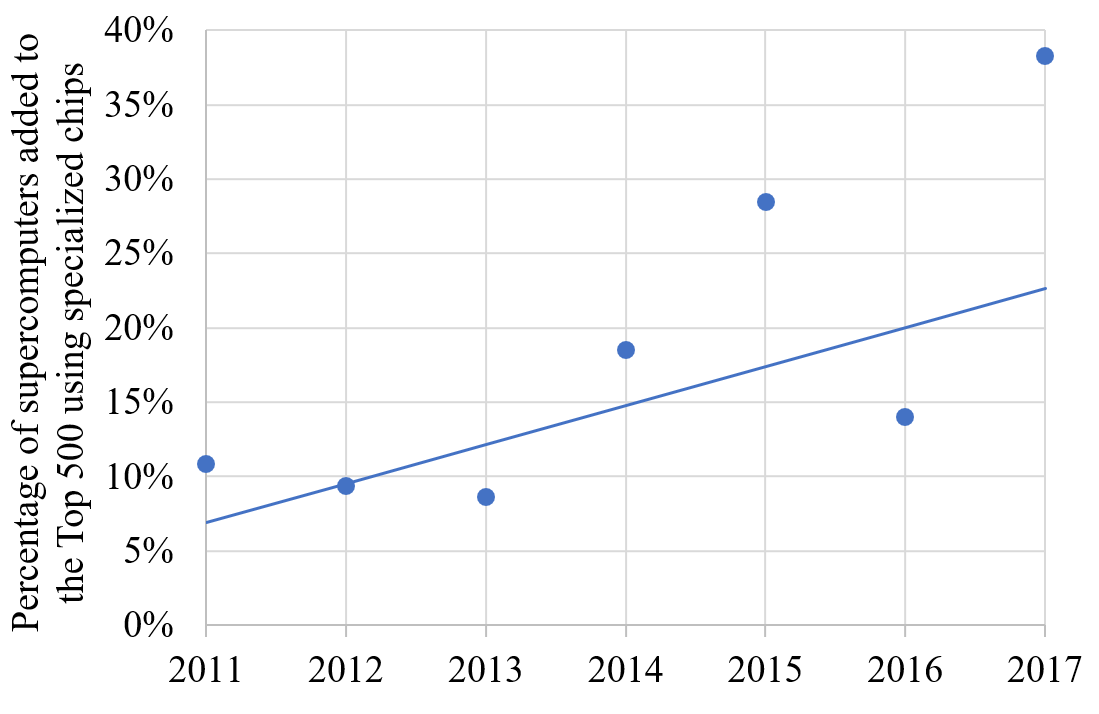
\includegraphics[scale=0.4]{figures/Supercomputers-with-pecialized-chips.png}
    \caption{Graph showing increasing popularity of 
specialized hardware in high performance computing \citep{GenPurpTech}}
    \label{fig:1}
\end{figure}

\section{FPGA Overview}
A field programmable gate array, or FPGA, is a digital integrated circuit that consists of millions of logic blocks that can be configured to perform different operations. The process of configuring the logic blocks is called FPGA design and can be compared to the design of integrated circuits. Reconfigurability and ease of design are the main advantages when using an FPGA as a computing platform. When comparing an FPGA design to a solution that is developed using software, the FPGA stands out with process pipelining and high a level of parallel processing. The difference between executing a software program on a processor and executing the equivalent operation on an FPGA is that the compiled software instructs the processor to do operations in a generic way, as in loading a register and shifting a bit. An FPGA does not need to explicitly load a register because the registers are by default connected to the input of the operation, which is defined by the FPGA design. A bit shift operation is typically an inexpensive operation regardless of the computing platform, but the FPGA can pipeline the result directly into another register or operation, which saves clock cycles \citep{XilFPGAIntro}.

% Volatile vs non volatile FPGA (SRAM, flash, anti-fuse)
% https://www.edn.com/a-comparison-of-space-grade-fpgas-part-1/
% https://www.edn.com/fpga-architectures-from-a-to-z-part-1/
% https://www.eetimes.com/all-about-fpgas/#
% FPGA Interconnect
% IO Cell, clocks http://xilinx.eetrend.com/files-eetrend-xilinx/forum/201509/9204-20390-7_series_architecture_overview.pdf
% https://nanopdf.com/download/fpga-programmable-interconnect-and-i-o-cells_pdf
% https://www.analog.com/en/analog-dialogue/articles/care-and-feeding-of-fpga-power-supplies-a-how-and-why-guide-to-success.html

\par
Xilinx is one of the key companies involved in FPGA production both currently and historically. They introduced the world to FPGAs in 1985 and have since then led the programmable logic technology industry with a 51\% market share of programmable logic device suppliers in 2017. Major end market categories for Xilinx are aerospace, defense, and communications. The main competitor of Xilinx is Intel with a market share of 37\% \citep{XilHist}\citep{XilShare}.
\par 
Due to the significance of Xilinx, and relevancy in this project, FPGA technology discussed in this work is Xilinx based. Differences between manufacturers includes technological and architectural nuances. For example, Xilinx exclusively manufactures static random access memory (SRAM) based FGPAs. This refers to the technology of the programmable parts of the FPGA. Other available tehcnologies are flash and anti-fuse, which are less common than SRAM \citep{FPGAarch1}.
\par
The basic internal elements of an FPGA consist of circuits such as look-up tables, flip-flops, wires, and input/output pads. Using these elements the FPGA design is implemented in the hardware.
The architecture is explained by Figure \ref{fig:2} which shows a matrix arrangement of configurable logic blocks which are connected to each other with the interconnect, consisting of wires and switch matrices. The wires also run to the input/output pads, which enables interfacing with off-chip components such as synchronous dynamic random access memory (SDRAM) or sensors \citep{XilFPGAIntro}. Configurable logic blocks (CLBs) contain the look-up tables and flip flops. An overview of a CLB is shown in Figure \ref{fig:3}.

\begin{figure}[h]
    \centering
    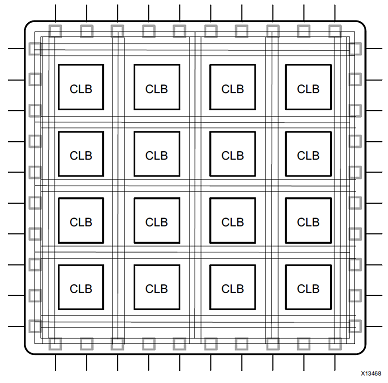
\includegraphics[scale=0.55]{figures/basic_fpga.png}
    \caption{FPGA architecture. An FPGA consist of configurable logic blocks, interconnect, and input/output pads \citep{XilFPGAIntro}.}
    \label{fig:2}
\end{figure}

\begin{figure}[h]
    \centering
    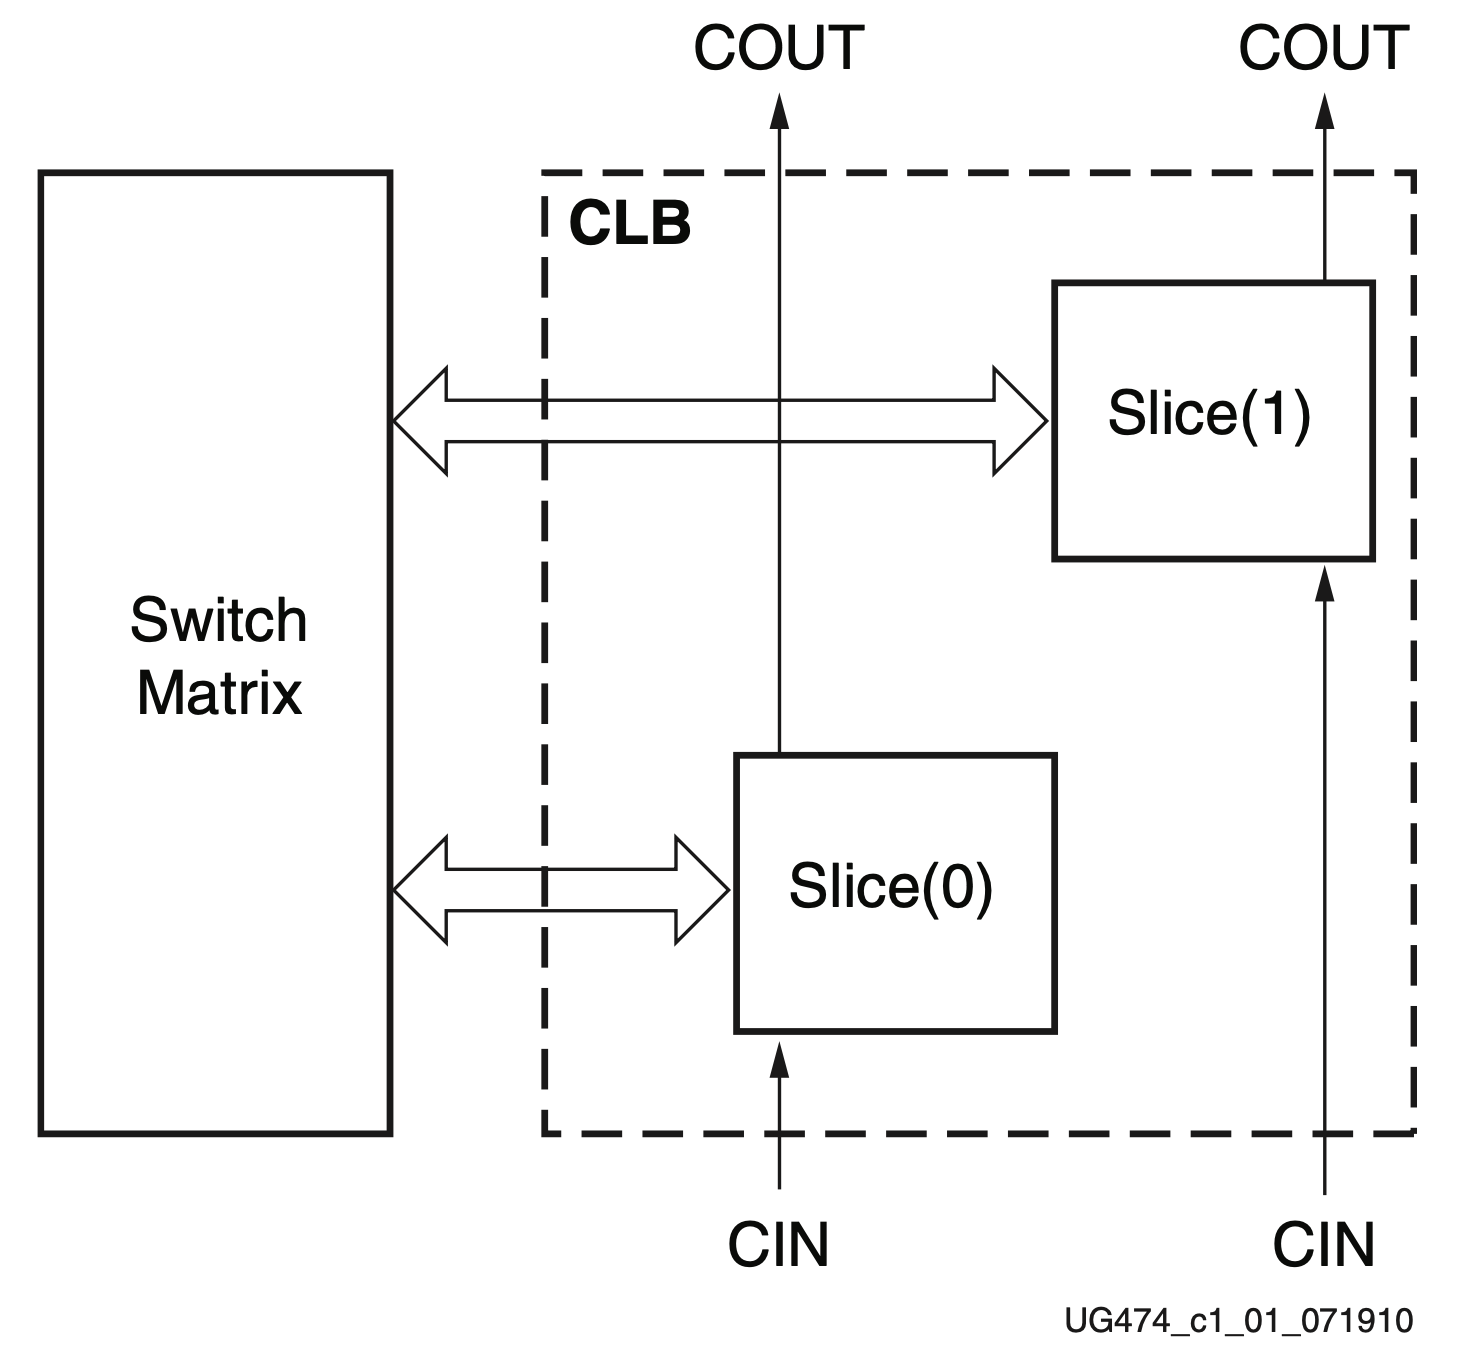
\includegraphics[scale=0.25]{figures/clb.png}
    \caption{Diagram of a configurable logic block. A CLB consists of logic element containers, called slices, inputs, and outputs. Both slices are attached to the switch matrix, connecting the CLB to other CLBs \citep{XilClbMan}.}
    \label{fig:3}
\end{figure}

The slices in Figure \ref{fig:3} represent core elements of an FPGA. Slices consist of look-up tables, storage elements, multiplexers, and carry logic. Depending on the FPGA there are different numbers of slices per CLB. The slices are collectively responsible for implementing a significant portion of the FPGA design \citep{XilClbMan}.
\par
Look-up tables, or LUTs, are mainly used as logic elements in FPGAs. They can implement any boolean logic operation by combining memory cells with multiplexers. The look-up table is essentially a truth table that can be used for reading the result of boolean operations. Memory cells and multiplexer routings are initialized by the FPGA design, which is what makes the look-up table element configurable \citep{XilFPGAIntro}. An example of a 4 memory cell wide LUT is shown in Figure \ref{fig:4}.

\begin{figure}[h]
    \centering
    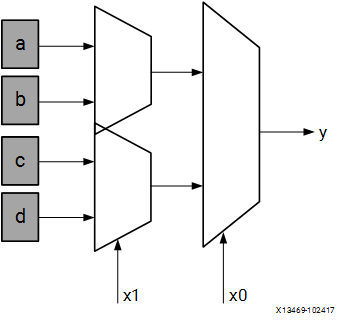
\includegraphics[scale=0.5]{figures/lut.png}
    \caption{Look-up table with 4 memory cells and two multiplexers. The FPGA design initializes memory cells \textbf{a-d} and uses inputs \textbf{x1} and \textbf{x0} to select value \textbf{y} \citep{XilFPGAIntro}}
    \label{fig:4}
\end{figure}

The circuit elements discussed in this chapter form the basic blocks of FPGA technology. A larger set of elements are often included in an FPGA to enable some optimizations and further functionality in the design. For example, there are different types of slices a CLB can contain, which makes it more suitable for storage purposes rather than logic. Signal processing pipelines are a popular use case for FPGAs and they often contain slices specialized for operations in this problem domain. Digital signal processing can be accelerated by parallelizing operations in a single instruction multiple data (SIMD) fashion, thus to maximize the advantage there can often be found a large number of these slices. Figure \ref{fig:5} shows an example of an FPGA configuration with some of these specialized blocks mapped out. The green CLBs are designated to memory usage and are closely coupled to the red digital signal processor (DSP) blocks to enable fast processing of the stored data. The purple external memory controllers use the input/output pads to interface with external memory such as SDRAM \citep{XilFPGAIntro} \citep{XilClbMan}.

\begin{figure}[h]
    \centering
    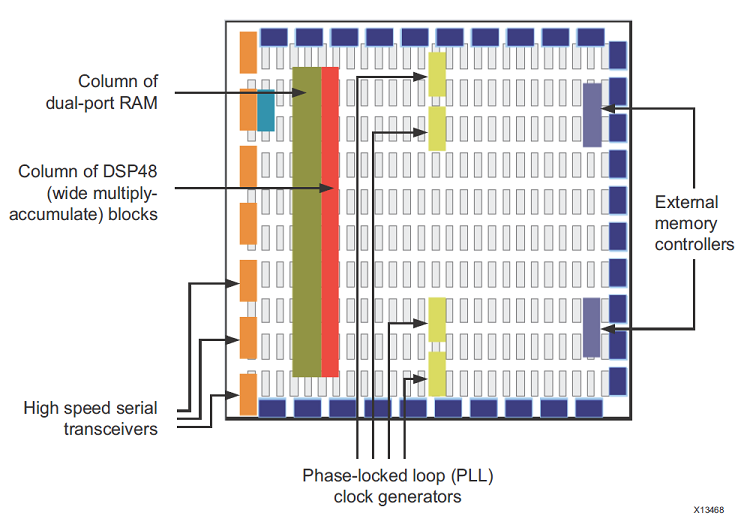
\includegraphics[scale=0.5]{figures/contemporary_fpga.png}
    \caption{DSP system design on FPGA \citep{XilFPGAIntro}}
    \label{fig:5}
\end{figure}

When comparing FPGAs with each other the main performance metrics are power consumption and number of logic cells. The number of logic cells determines the size and complexity of the design that the FPGA can fit. Additionally, the FPGAs can often be compared by specifications such as specialized CLB slices, IO interfaces, and communication rates. Clock speed is seldom compared because although there is an upper limit, it is often design specific \citep{XilClbMan} \citep{XilFPGAIntro}. 

\section{System design with HDL}
The main tool for creating an FPGA design is a hardware description language (HDL). VHDL and Verilog are examples of commonly used HDLs. Compared to conventional computer programming languages, HDLs are used in a data flow fashion to describe the timing and logic of an integrated circuit. The data flow description of a circuit in an HDL is such that all code blocks are executed simultaneously by default. This is one of the main advantages of FPGAs as the system is inherently parallelized. It creates also one of the biggest challenges in HDL based design as it complicates the timing of events and resource concurrency.
\par
The output of an HDL design is produced by a build process that computes the high level data flow description into low level circuit elements and routing. This can be compared to the compilation phase of code written in a statically typed software programming language. 
\par
The synthesis process is where the HDL design known as register transfer level code is transformed to a gate level description called netlist. The netlist is a mapping of circuit components that are found inside the FPGA. The convenience of HDL based design is being able to describe the circuit at a higher level. In practice this means that registers and buses are created and connected to be inferred into low level circuitry at the synthesis phase. When developing a design against a specific FPGA, a bitstream file is created to configure the device with. The end product of an HDL based design is the bitstream file or, alternatively, the synthesis result as it can be used for simulation purposes by a test bench \citep{XilVivado}.

\section{System design with IP cores}
Designing a hardware system often involves components of a reusable nature, such as dividers, communication protocols, and memory controllers. Intellectual property (IP) cores are distributions of components such as these. An IP core can be of varying complexity as it can consist of a solution for a specific task or describe a complete system on a chip (SoC). IP cores are licensed through a patented design which is what the name refers to. They can often be configured to suit different properties of the implementation such as data width and clock rate. The core is then connected to the system using an HDL. The core itself may consist of software or hardware macros. The software macro, or soft IP core, is an HDL implementation of the IP core logic that is built to the specific FPGA with the rest of the system design. A hardware macro, or hard IP core is prebuilt and FPGA specific \citep{EERefBook} \citep{XilVivado}.
\par
The hardware sector and consumer electronics industry rely heavily on reusable IP cores. For example, the SoC or motherboard found in mobile phones often include advanced RISC machine (ARM) based processor cores licensed from ARM holdings. The producer of the mobile phone benefits from avoiding the development of the processing unit but still has the ability to customize the SoC to a high degree by combining different processing units, memories, and other IP cores \citep{ArmInMobile} \citep{HarvIPCore}. Figure \ref{fig:6} shows the architecture of a SoC which has an ARM based CPU, and other modules commonly found in mobile phones. In addition to the CPU, any of the remaining modules might also be licensed IP cores.

\begin{figure}[h]
    \centering
    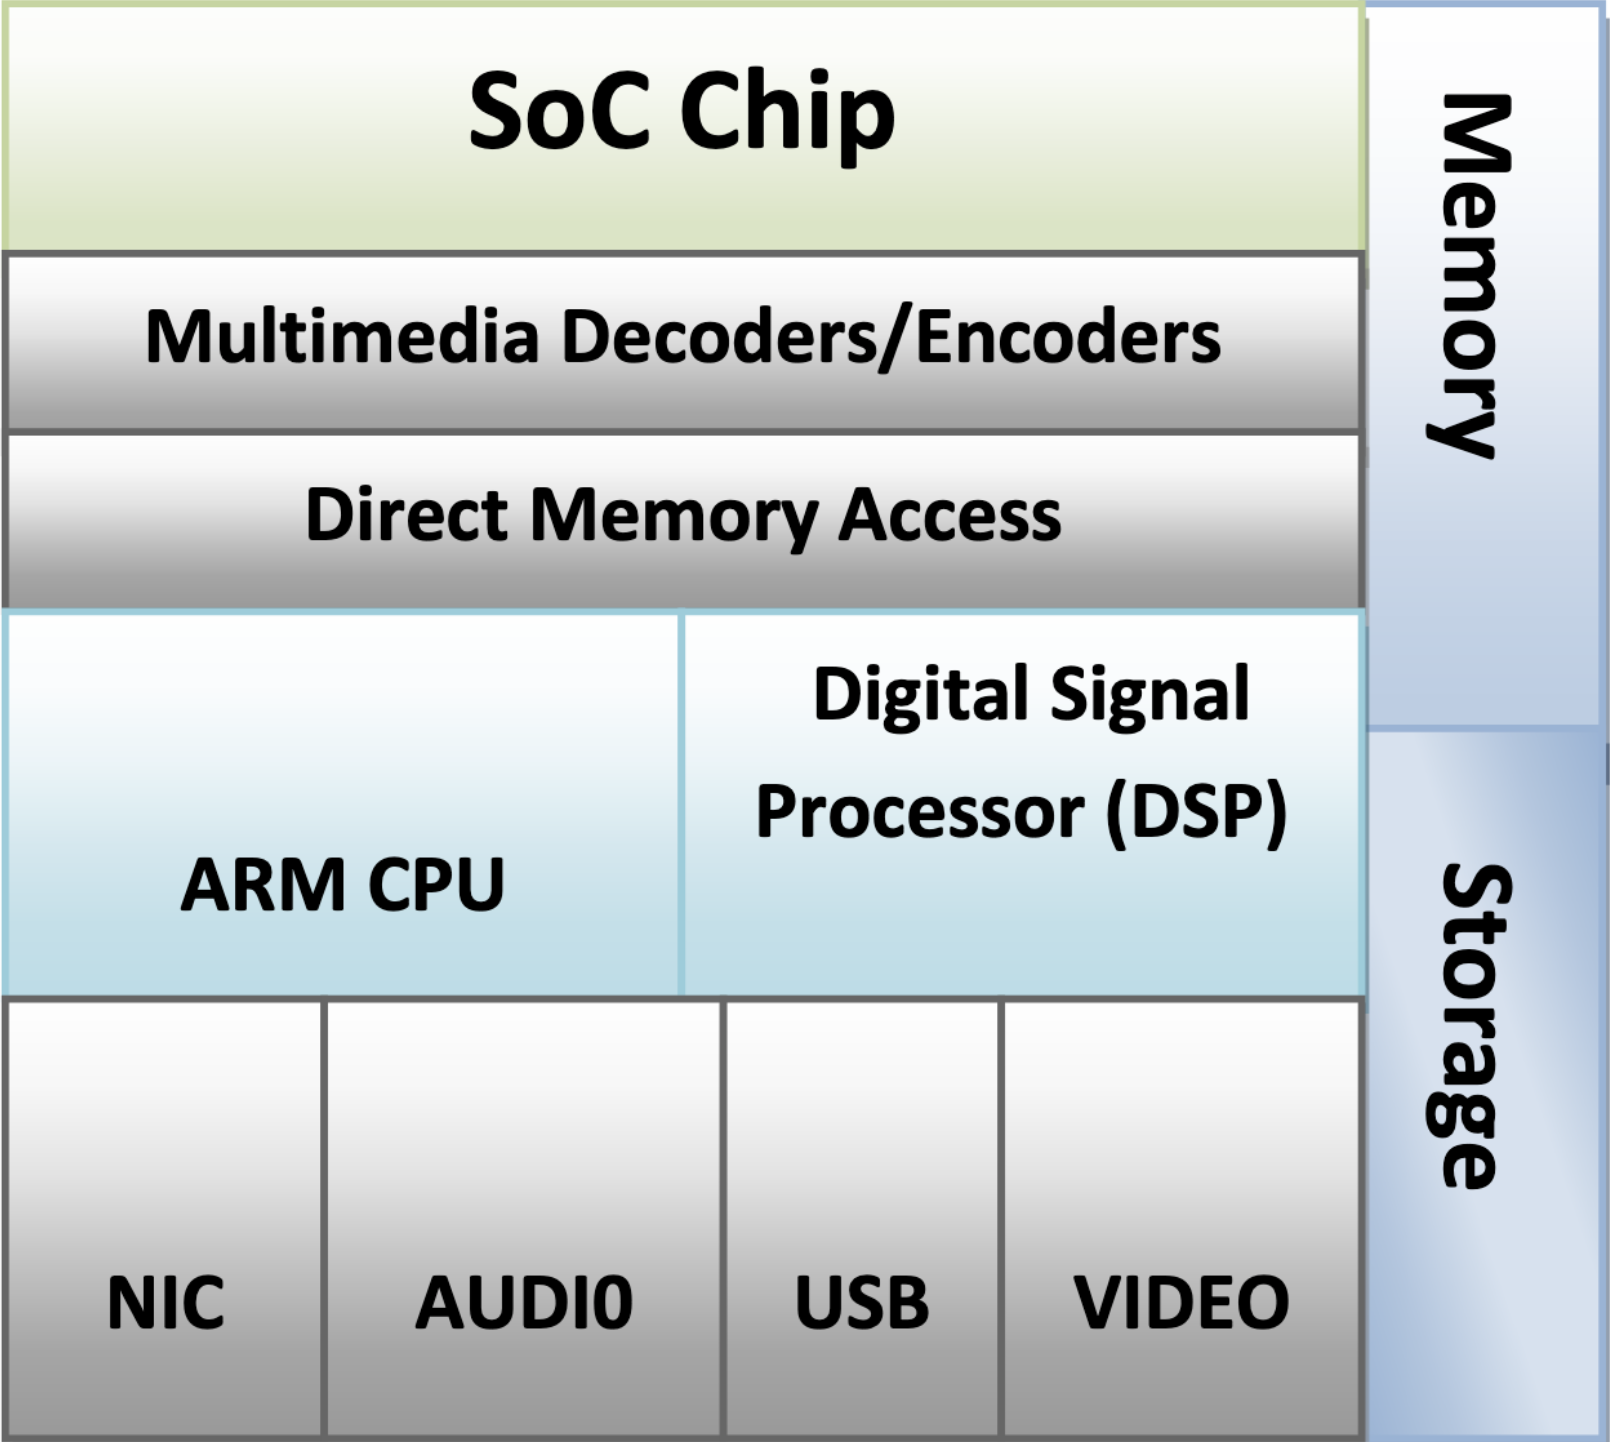
\includegraphics[scale=0.25]{figures/arm_soc.png}
    \caption{Common SoC found in smartphones includes ARM based CPU and a DSP. \citep{ArmInMobile}}
    \label{fig:6}
\end{figure}

\par
In aerospace applications, the advantages of IP cores are utilized in the same manner as within the mobile phone industry. Additional requirements such as fault tolerance limits, redundancy, and formal verification of the IP cores increase the advantages of their usage when comparing to in-house developed solutions. This, however, comes with pricier licenses compared to non-aerospace grade IP core designs. Also, due to the specialized requirements, lower competition in the market sector can be expected, increasing the prices even more \citep{DO254Cadence}.
\par
In addition to FPGA products, Xilinx also provides design tools and IP cores to help with development on their FPGA platforms. Their IP core library ranges from common IC to complete microcontrollers. Some of the cores are available free to use through the Vivado design suite, and a majority of them are soft cores to allow compatibility across their FPGAs. Integration of the IP cores and other development is also done through Vivado \citep{XilVivado}.
%OPENCORES
% https://www.xilinx.com/content/dam/xilinx/support/documentation/white_papers/wp523-xqrku060.pdf
% https://www.techspot.com/article/1989-arm-inside/
% https://www.techspot.com/article/1821-how-cpus-are-designed-and-built/
%The image processing pipeline uses three different storage mechanisms. 
%\subsection{SDRAM}
%The main working memory of the image processing pipeline is a off-chip 512MiByte, 32-bit wide DDR3 SDRAM memory module.
%\subsection{BRAM}
%\subsection{FIFO}
%\subsection{PipeIn/PipeOut}

%\section{Licensing and standards}
%\subsection{IEEE}
%\subsection{ISO}
%\subsection{DO-254}
% https://www.cadence.com/content/dam/cadence-www/global/en_US/documents/solutions/aerospace-and-defense/do-254-explained-wp.pdf
% https://people.duke.edu/~goodw010/Wiki/hwswstds.html
%\subsection{MIL}

\chapter{System requirements}

A hardware implementation of an image analysis software component is to be developed to be used on an FPGA. The software in question is a product of a European space agency funded research project regarding detection and analysis of space debris in low earth orbit. Using computer vision among other analysis, space debris is identified from image data. With the help of a star catalog the image is mapped to a position in space to provide positional data of the detected debris. A diagram of the system is shown in Figure \ref{fig:0}. The software component relevant to this project is the Pre-processing \& Segmentation part of the diagram, which is in the input phase of the complete system \citep{StreakDet} \citep{Starmatch}.

\begin{figure}[h]
    \centering
    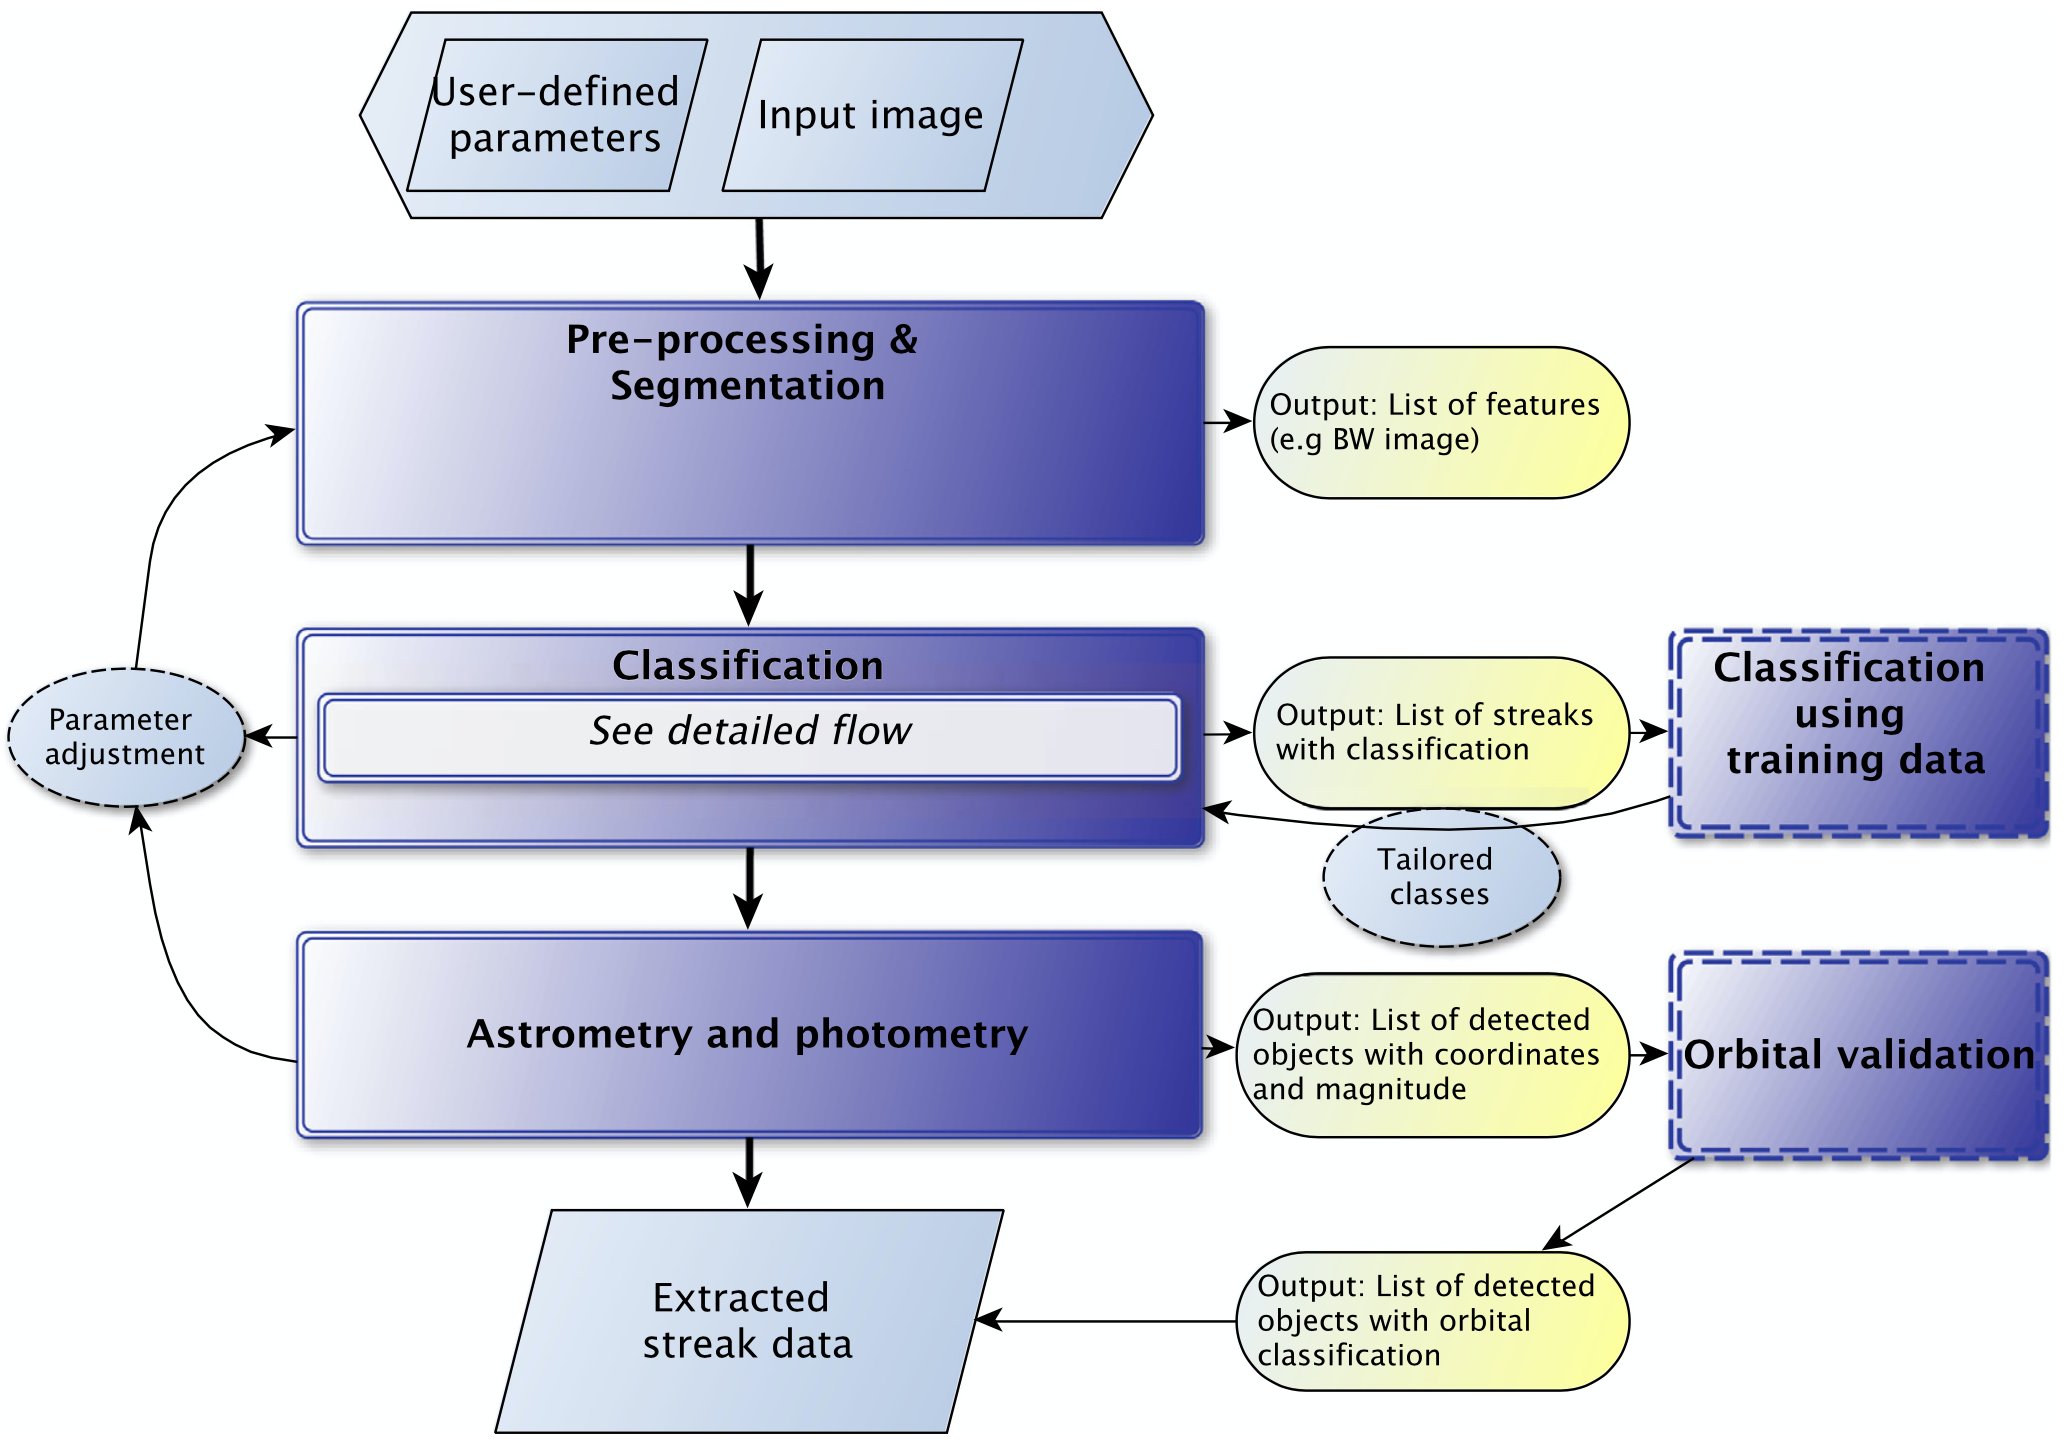
\includegraphics[scale=0.2]{figures/streakdet.png}
    \caption{Flowchart of StreakDet software \citep{StreakDet}}
    \label{fig:0}
\end{figure}

%\section{Scope}
The star extraction process in StreakDet passes the input image through a series of algorithms to identify stars. The algorithms are well known image filters and analysis methods that in combination with each other produce a way to pick out objects from an image. The main task in this project is to identify these algorithms and fit them into a hardware design using a hardware description language.
\par
Star extraction is a key stage of a star tracker system which uses a star catalog to match the extracted stars against. Using the star matches and catalog information the position and orientation of the captured image can be determined. The goal of this project is to create a pre-processing pipeline to be used in a star tracker.

\section{System specification}

The specification consists of development and system requirements as well as a description of tools and components. System requirements are created based on meetings and discussions with Aboa Space Research Oy. Some requirements are derived from higher level requirements to suit the development process. Table \ref{table:1} presents an overview of the system in a functional and non-functional requirements fashion.

\begin{table}[h]
    \begin{tabular}{|p{1cm}|p{6.15cm}|p{6.15cm}|}
        \hline
        \textbf{Req. Id}& \textbf{Functional requirement}& \textbf{Non-functional requirement}\\
        \hline
        1&The FPGA is used as processing node for extracting stars from an optical image&Convert StreakDet star extraction software algorithm to a hardware design\\
        \hline
        2&A communication channel is available for shared memory usage&FPGA implements memory controller interface and USB port controller\\
        \hline
        3&Allow configuration of processing pipeline parameters&Frontend software is used for pipeline configuration\\
        \hline
        4&Processed images and intermediate results can be verified&Pipeline stage results are written to storage\\
        \hline
        5&Performance metrics of process and stages can be viewed&Pipeline captures and stores metrics along the stages\\
        \hline
    \end{tabular}
    \caption{Table of functional and non-functional system requirements}
    \label{table:1}
\end{table}

%The development requirements involves critical steps that are necessary when working towards the system requirements.
%\subsection{Scope}
%\subsection{Image processing pipeline stages}
\subsection{System components}
\subsubsection{Processing nodes}
The system consists of two nodes, the host machine and the target FPGA. Because the application of this system will be different in a production environment, the FPGA part should not be too dependent on the host machine. When integrated into a larger system with shared memories and communication, the FPGA will have to be able to read an input image directly from memory. The same applies to the output, the register where the output is written needs to be configurable and not sent to a host machine by default.

\subsubsection{FPGA module}
The FPGA module Opal Kelly XEM7305 chip with a Xilinx Spartan-7 FPGA will function as a testbed for development. The module contains a part from the FPGA external SDRAM memory and communication interfaces such as USB 3. These features allow for host machine communication and data storage of features such as images, star catalog, and output. These data could be stored on the FPGA itself but using the SDRAM is a sustainable solution because it allows for shared memory usage in production and more flexible image and star catalog sizes.


\chapter{FPGA based computer hardware}
Common computer hardware is the corner stone of any digital circuit that needs to perform common tasks such as storing and transmitting data. With the help of the basic elements of an FPGA discussed in Chapter 2, circuits of this nature can be created. Although an 8-bit adder circuit can be regarded as common computer hardware, the focus of this chapter is on larger circuits used as hardware modules such as memory and communication interfaces. The components discussed are essential building blocks for the image processing pipeline.

\section{Communication}
The system requirements state a communication channel to be available for shared memory usage and controlling the FPGA. Machine to machine communication is enabled trough the interfaces available on the Opal Kelly FPGA module. The default interface on XEM7305 is USB 3.
\par
The advantage of the USB standard in general is flexibility and ease of use. Transfer speed is not a high priority in this case because of the relatively small size of data, which is less than a megabyte. The USB module on the XEM7305 contains the port itself and a Cypress FX3 microcontroller which is exposed to various systems on the FPGA module. The HDL interface of the USB controller is a hard IP core.
\par
Internally, the FPGA uses communication channels defined by the HDL. The limiting factor and bottleneck is often some hardware module that places certain requirements on the communication, for example the USB3 or memory controller. When working outside these types of dependencies, the throughput of the system can be optimized by maximizing the bit width between modules. When applying this to the image processing pipeline context, this might be practical within communication of image data. The implementation of this requires more memory cells and wires, which in turn increases the footprint of the FPGA design.
\par
When comparing to a software program, the same optimization method of maximizing bit width might be considered. This, however, does not inherently result in a gain in throughput because conventional CPUs have a fixed bit width for their operations. When this limit is exceeded the operation needs to be performed across multiple clock cycles which counteracts the wanted result. The bit width of an operation on an FPGA during a clock cycle is consistent with the HDL definition. 

% Image of low vs high bit width circuit/ footprint
% More in depth on USB3, images
% https://www.usb.org/sites/default/files/CabConn_3_0_Compliance_Document_20101020.pdf
% https://www.usb.org/documents?search=&category%5B%5D=49&tid_2%5B%5D=39&items_per_page=50
% PipeIn PipeOut
% Cypress FX3 Microcontroller

\section{Memory}
To enable processing of image data, a set of storage mechanisms is necessary. The dependence to a mechanism is mostly based on the size of the data and how it will be used. As in conventional CPU architectures, different levels of memory are used to satisfy these dependencies.
\par
FPGAs are generally not well suited for storing a large quantity of data as it is considered inefficient use of available CLBs. Since customization is a key feature, the most standardized parts, such as memory, are often placed outside the FPGA. Off chip memory allows storage of large data, such as images, freeing up CLBs to other usage such as computation and logic. The downside with off chip components is them often being a bottleneck in the system. This is due to a number of factors such as restrictions in clock speed, concurrency, and bus width. A larger FPGA with an increased number of CLBs could offset the need for off chip memory avoiding the bottleneck, with consequences being greater power consumption and physical size, potentially invalidating the solution.

\subsection{SDRAM}
One of the most common storage mechanisms is SDRAM which is useful to store data that is frequently used and ranges from kilobytes to megabytes in size. Key features include random access, meaning same access time for any part of the memory, and high bandwidth. It is often paired with FPGAs because it is next in the memory hierarchy after on chip storage mechanisms.
\par
At the core of SDRAM lie capacitors trapping the charge representing a bit. An overview of a typical SDRAM circuit is shown in Figure \ref{fig:7}. The capacitors are refreshed periodically to retain the stored data. This makes SDRAM a volatile memory, requiring power to keep its state. The advantage over closely related memory types such as flash memory, is that it does not degrade at the same rate of read/write cycles and it is truly random access, giving the advantage to SDRAM as a volatile working memory in most FPGA applications \citep{SDRAMFLASH} \citep{NANDNORFlash}.

\begin{figure}[h]
    \centering
    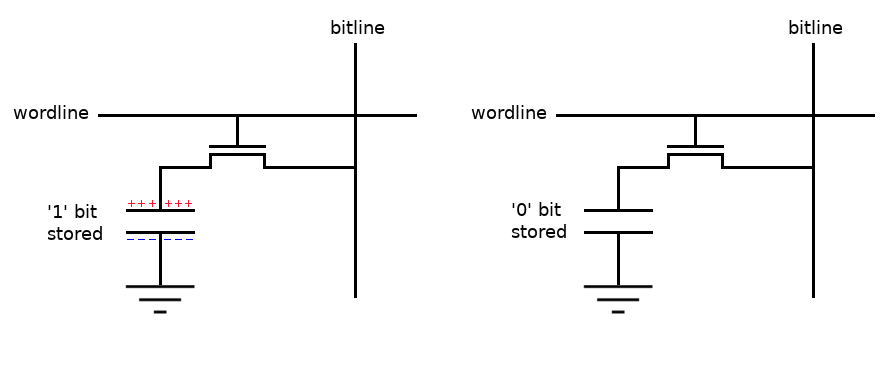
\includegraphics[scale=0.4]{figures/DRAM.jpg}
    \caption{SDRAM memory cell. The capacitor traps the charge which is controlled by the transistor at the top \citep{SDRAMFLASH}.}
    \label{fig:7}
\end{figure}

The memory cells in SDRAM are ordered in rows and columns, forming an array. A collection of these arrays are referred to as memory banks. 
\begin{wrapfigure}{r}{0.5\textwidth}
    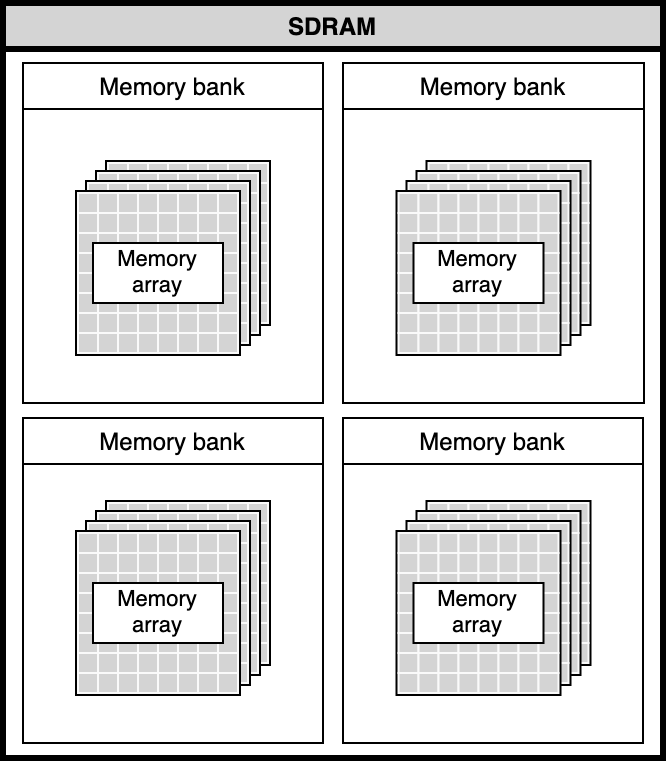
\includegraphics[scale=0.3]{figures/sdram_bank_array.png}
    \caption{SDRAM geometry.}
    \label{fig:8}
\end{wrapfigure}
The number of rows, columns, arrays, and banks varies depending on the type of SDRAM, but is usually a power of 2. Figure \ref{fig:8} shows the geometry of an SDRAM with 4 banks with 4 arrays each. The data width of a memory is the number of arrays that are stacked inside each memory bank. When accessing a specific row and column, the number of affected bits is the same as the data width of the memory.
\par
To increase SDRAM performance, double data rate (DDR) is used to access data at double the clock rate. DDR enables accessing a memory bank on both the rising and falling edge of the clock cycle. A prefetch mechanism enables the transfer of multiple bits concurrently per bank access, increasing the throughput even more. This mechanism enables efficient use of the internal SDRAM bus width by also transferring data from neighboring addresses. The gain comes from the fact that the time to access a single address is the same as accessing the neighboring ones as well. The prefetch mechanism gives an advantage to data which is structured in a way where each access is in adjacent addresses. The width of the prefetch data depends on the DDR version. Other variations between DDR versions are the supported clock frequency and burst length, which is a feature related to the prefetch mechanism. The burst length specifies the number of SDRAM words contained in each read or write operation \citep{MicronSDRAMGeneral}.
\par
The XEM7305 features a Micron DDR3 SDRAM chip with a 32-bit wide interface. The memory part has 8 banks, 32 000 row addresses, 1000 column addresses, and 16 bits to each address, giving the a capacity of 4Gb. As previously discussed, the DDR version dictates the prefetch data width, which in DDR3 is 8 words, as is the burst length. The word length of the memory is 16 bit, which results in 128-bit burst transfers. The SDRAM is rated with a clock frequency of 1600 MHz, giving a theoretical peak bandwidth of 3.2 GB/s. In practice, the bandwidth is lower and depending on system state and access location \citep{XEM7305Man}.
\par
The oscillator on the FPGA board provides a 200 MHz signal, which is also the limit of the Spartan 7 FPGA. This allows a maximum clock frequency of 325 MHz to be generated through the SDRAM controller interface and then scaled up to 650 MHz with DDR at the SDRAM.
\citep{XEM7305Man} \citep{MicronSDRAM}.
\par
The memory controller interface connects the FPGA to the SDRAM controller, which in turn sends commands to the SDRAM core. The interface is unique to each memory controller and depends on all parameters discussed in this chapter such as memory geometry, DDR version, and clock frequency \citep{XEM7305Man}.

%((32k * 1k)*8) = addr
%addr * 16 = capacity

%https://www.xilinx.com/support/documentation/user_guides/ug473_7Series_Memory_Resources.pdf
%https://user.eng.umd.edu/~blj/memory/Book-Overview.pdf
%https://www.allaboutcircuits.com/technical-articles/executing-commands-memory-dram-commands/
%http://taututorial.yolasite.com/sdram-controller.php
%https://itectec.com/superuser/how-to-interpret-the-parameters-in-a-dimm-datasheet/
%https://www.micron.com/-/media/client/global/documents/products/technical-note/dram/tn4605.pdf
%https://www.es.ele.tue.nl/premadona/files/akesson01.pdf
%https://www.design-reuse.com/articles/13805/the-love-hate-relationship-with-ddr-sdram-controllers.html

\subsection{Block RAM}
When data size is within a few megabytes or less, lower level storage mechanisms become suitable to use as memory. The block random access memory (BRAM) is a type of on-chip memory, which uses memory cells available on the FPGA. The specification of an FPGA chip often include the available BRAM capacity. Although BRAM is a type of on-chip memory, it is separate from the CLBs on the FPGA. In the case of SRAM based FPGAs, the memory cells of the BRAM are essentially SRAM cells, arranged in arrays. The BRAM is made available to the other CLBs by being attached to the FPGA interconnect.
\par
BRAM can be configured in size and functionality depending on the needs. Common BRAM arrays are 36Kb, that can either be divided into smaller arrays, or combined with other arrays to form a larger memory resource. A useful feature often found regarding BRAM is multi port support. This enables concurrent usage of the memory resource. In case of concurrency issues, the configurable operation mode of the BRAM dictates how to resolve them. For example, in a dual port configuration, the read first operation mode will prioritize a read operation when the other port requests a write operation on the same address.
\par
% example configuration & geometry
\par
Similarly as SDRAM, BRAM also is synchronous and requires a clock signal. The latency is depending on the configuration and state of the memory, but usually within a few clock cycles. The low latency, together with the high configurability makes BRAM a useful resource in most FPGA designs.

% shift register vs block ram
% https://www.xilinx.com/support/documentation/white_papers/wp377_7Series_Embed_Mem_Advantages.pdf
% https://eprint.iacr.org/2018/717.pdf
% https://archive.org/details/eu_SciAm_1997-06_OCR/page/n55/mode/2up?q=configurable+computing+scientific+america
% http://www.righto.com/2020/09/reverse-engineering-first-fpga-chip.html
% https://ieeexplore.ieee.org/document/6487750?reload=true
% https://www.xilinx.com/support/documentation/ip_documentation/blk_mem_gen/v8_3/pg058-blk-mem-gen.pdf
\subsection{Distributed RAM}

\section{Computation}
% clocks, dsp, bitwidth etc.
\chapter{FPGA based data structures and algorithms}

\chapter{Documentation}

\section{Pipeline algorithms}
\subsection{Box Filter}
\subsection{Thresholding}
\subsection{Connected component labeling and analysis}

\chapter{Development process}

\chapter{Review and reflection}

\chapter{Discussion}

%\section{Space grade hardware design}

\addcontentsline{toc}{chapter}{Bibliography}

\bibliographystyle{unsrt}
\bibliography{references}

\end{document}
